\chapter{Рубежный контроль}
\label{cha:analysis}

\section{Постановка задачи}
\label{sec:task}
Оптимизировать код кластеризации методом k-means, не задействуя массивов, кроме массива расстояний от одной точки до каждого центроида и массива номеров кластеров длиной M, где M - количество трёхмерных точек на входе алгоритма (точки для работы можно нарандомить).

\section{Решение}
\label{sec:solution}
Кластеризация методом k-средних состоит из нескольких этапов:
\begin{enumerate}
	\item Инициализировать центры кластеров;
	\item для каждой точки найти минимальное расстояние до центроида;
	\item установить принадлежность точки соответствующему кластеру;
	\item Вычислить новые центроиды, как среднее всех точек кластера.
\end{enumerate}
Шаги 3 и 4 повторяются до тех пор, пока не будет достигнуто условие остановки, в моём решении это достижение предела количества итераций.
\par В листинге \ref{code:center} приведена функция поиска ближайшего центроида для каждой точки и присваивание точки кластеру.
\begin{lstlisting}[caption= Функция поиска ближайшего центроида, label=code:center]
	void closest_center(point* points, int npoints, point* centers, int k, int* clusters)
	{
		for (int i = 0; i < npoints; i++)
		{
			float min = 150 * 150 * 150;
			int cluster = 0;
			for (int j = 0; j < k; j++)
			{
				float d = distance(points[i], centers[j]);
				if (d < min)
				{
					cluster = j;
					min = d;
				}
			}
			clusters[i] = cluster;
		}
	}
\end{lstlisting}
В листинге \ref{code:unopt} представлена функция кластеризации точек по кластерам k, для возможности дальнейшего сравнения алгоритмов центры передаются инициализированными.
\begin{lstlisting}[caption= Не оптимизированная функция кластеризации, label=code:unopt]
int* clustering(point* points, int npoints, int k, point* centers)
{
	int* clusters = new int[npoints];
	
	for (int iter = 0; iter < ITERATIONS; iter++)
	{
		closest_center(points, npoints, centers, k, clusters);
		
		for (int i = 0; i < k; i++)
		{
			centers[i].x = 0;
			centers[i].y = 0;
			centers[i].z = 0;
		}
		
		for (int i = 0; i < npoints; i++)
		{
			centers[clusters[i]].x = centers[clusters[i]].x + points[i].x;
			centers[clusters[i]].y = centers[clusters[i]].y + points[i].y;
			centers[clusters[i]].z = centers[clusters[i]].z + points[i].z;
		}
		
		for (int i = 0; i < k; i++)
		{
			int cl = 0;
			for (int j = 0; j < npoints; j++)
			if (clusters[j] == i)
				cl = cl + 1;
			
			if (cl)
			{
				centers[i].x = centers[i].x / float(cl);
				centers[i].y = centers[i].y / float(cl);
				centers[i].z = centers[i].z / float(cl);
			}
		}
	}
	
	return clusters;
}
\end{lstlisting}

В листинге \ref{code:opt} представлена оптимизированная функция кластеризации.
\begin{lstlisting}[caption= Оптимиpированная функция кластеризации, label=code:opt]
int *clustering_opt(point *points, int npoints, int k, point *centers)
{
	int *clusters = new int[npoints];
	
	for (int iter = 0; iter < ITERATIONS; iter++)
	{
		closest_center(points, npoints, centers, k, clusters);
		
		for (int i = 0; i < k; i++)
		{
			centers[i].x = 0;
			centers[i].y = 0;
			centers[i].z = 0;
			
			int cl = 0;
			for (int j = 0; j < npoints; j++)
			{
				if (clusters[j] == i)
				{
					cl++;
					centers[i].x += points[j].x;
					centers[i].y += points[j].y;
					centers[i].z += points[j].z;
				}
			}
			if (cl)
			{
				centers[i].x /= float(cl);
				centers[i].y /= float(cl);
				centers[i].z /= float(cl);
			}
		}
	}
	
	return clusters;
}
\end{lstlisting}
С целью оптимизации были приняты такие меры:
\begin{enumerate}[1.]
	\item где это возможно операторы формата $a = a + b$ заменены на $a+=b$ или аналогичные;
	\item объединены циклы, связанные с вычислением новых центроидов, а именно:
	\begin{enumerate}
		\item цикл зануления координат центроида;
		\item цикл суммирования значений центроида;
		\item цикл подсчёта размерности кластера;
	\end{enumerate}
	\item слияние циклов позволило избавится от сложной индексации в суммировании координат.
\end{enumerate}

\subsection{Рассчитаем трудоёмкости}
\label{subsec:hard}
Расчёт будем производить только для изменённой части.
\par Не оптимизированная функция:
\begin{equation}
\begin{split}
	&f=2+k*(2+6)+2+n*(2+12+3+3+3)+2+\\
	&k*(2+1+2+n*(2+2+\begin{cases}
		2\\0
	\end{cases})+1+\begin{cases}
	6+3+3\\0
	\end{cases})=\\
	&=6+8k+23n+k*(6+\begin{cases}
		9\\0
	\end{cases}+n*(4+\begin{cases}
	2\\0
	\end{cases}))\\
	&=kn(4+\begin{cases}2\\0\end{cases})+23n+k(14+\begin{cases} 9\\0\end{cases})+6
\end{split}
\end{equation}
\par Оптимизированная:
\begin{equation}
\begin{split}
	&f=2+k*(2+6+1+2+n*(2+2+\begin{cases}1+6+3\\0\end{cases})+1+\begin{cases}3+3\\0\end{cases})=\\
	&=2+k*(12+n*(4+\begin{cases}9\\0\end{cases})+\begin{cases}6\\0\end{cases})=\\
	&=kn(4+\begin{cases}9\\0\end{cases})+k*(12+\begin{cases}6\\0\end{cases})+2
\end{split}
\end{equation}
\section{Тестирование}
\label{sec:tests}
Тестирование проводилось на случайно генерируемых массивах точек, координаты которых лежат в пределах от -100 до 100 по каждой размерности. Результатом работы программы является: массив номеров кластеров -- номер кластера указывает к какому кластеру принадлежит i-ая точка. И множество центроидов. Тесты проводились для 20 точек и 3 кластеров, 30 точек и 7 кластеров, 35 точек и 10 кластеров. 
\par На рисунках \ref{fig:screenshot001}-\ref{fig:screenshot003} представлены примеры работы программы.
\begin{figure}[H]
	\centering
	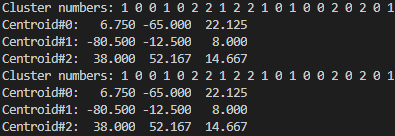
\includegraphics[width=0.5\linewidth]{src/screenshot001}
	\caption{Пример работы}
	\label{fig:screenshot001}
\end{figure}
\begin{figure}[H]
	\centering
	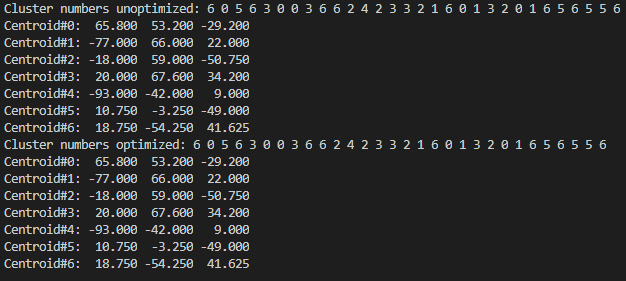
\includegraphics[width=0.5\linewidth]{src/screenshot002}
	\caption{Пример работы}
	\label{fig:screenshot002}
\end{figure}
\begin{figure}[H]
	\centering
	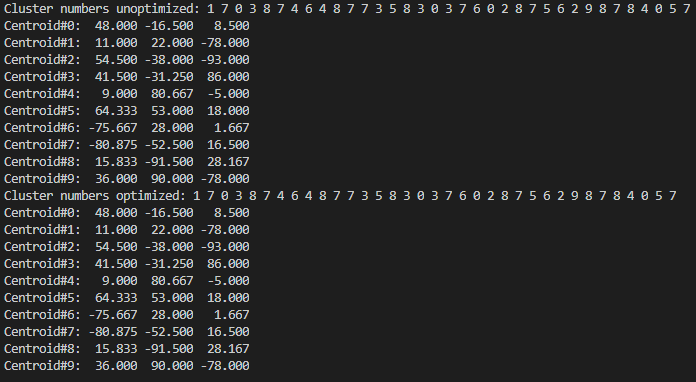
\includegraphics[width=0.7\linewidth]{src/screenshot003}
	\caption{Пример работы}
	\label{fig:screenshot003}
\end{figure}
Все тесты пройдены успешно.



\section{Вывод}
\label{sec:res}
Был оптимизирован код алгоритма кластеризации методом k-средних. 